\documentclass[a4paper,11pt, twoside]{book}

\usepackage[utf8]{inputenc}

\usepackage{graphicx}

\usepackage[indonesian]{babel}

\usepackage{geometry}
\geometry{inner=2.5cm, outer=2cm, top=2cm, bottom=3cm}

\usepackage{hyperref}

\usepackage{enumitem} %
\newlength\docparskip
\parskip=6pt
\setlength{\docparskip}{\parskip}
\setlist{nosep, itemsep=0pt, parsep=0pt, before={\parskip=0pt}, after=\vspace{-\docparskip}}%

\usepackage{amsmath}

\usepackage{amsthm}
\theoremstyle{definition}
\newtheorem{exmp}{Contoh}[section]

\usepackage{fancyhdr}
\fancyhf{} % clear all header and footers
\renewcommand{\headrulewidth}{0pt} % remove the header rule
\fancyfoot[LE,RO]{\thepage} % Left side on Even pages; Right side on Odd pages
\pagestyle{fancy}
\fancypagestyle{plain}{%
	\fancyhf{}%
	\renewcommand{\headrulewidth}{0pt}%
	\fancyhf[lef,rof]{\thepage}%
}

\usepackage[font=footnotesize]{caption}

\begin{document}
	
	\author{Mifta Nur Farid, M.T.}

	\title{Buku Ajar\\
		Rangkaian Elektronika II}

	\date{Januari 2021}
	
	\frontmatter

	\maketitle

	\tableofcontents
	
	\mainmatter
	
	\chapter{Differential Amplifier}
	\chapter{Operational Amplifier}

\section{Tujuan Pembelajaran}

Setelah mempelajari bab ini, kalian diharapkan mampu untuk

\begin{enumerate}
	\item Menjelaskan karakteristik dari op amp ideal dan op amp 741.
	\item Menentukan \textit{slew rate} dan menggunakannya untuk mencari \textit{power bandwidth} dari op amp.
	\item Menganalisis op amp inverting amplifier.
	\item Menganalisis op amp noninverting amplifier.
	\item Menjelaskan cara kerja summing amplifier dan voltage follower.
	\item Menjelaskan IC linear lainnya dan mendiskusikan bagaimana penggunaannya.
\end{enumerate}

\section{Pengantar Op Amp}

Gambar \ref{fig:16.01} menunjukkan diagram blok dari op amp. \textit{Input stage} dari op amp tersebut adalah diff amp, kemudian dilanjukan oleh lebih banyak \textit{stage gain}/ penguat, dan sebuah \textit{Class-B push-pull emitter follower}. Karena diff amp berfungsi sebagai \textit{first stage}, maka diff amp yang akan menentukan karakteristik \textit{input} dari op amp. Pada sebagian besar op amp memiliki \textit{output} berupa \textit{single-ended}. Dengan positif dan negatif \textit{supply}, \textit{single-ended output} didisain untuk memiliki nilai diam (\textit{quiescent value}) nol. Artinya, tegangan \textit{input} nol idealnya menghasilkan tegangan \textit{output} nol.

\begin{figure}
	\centering
	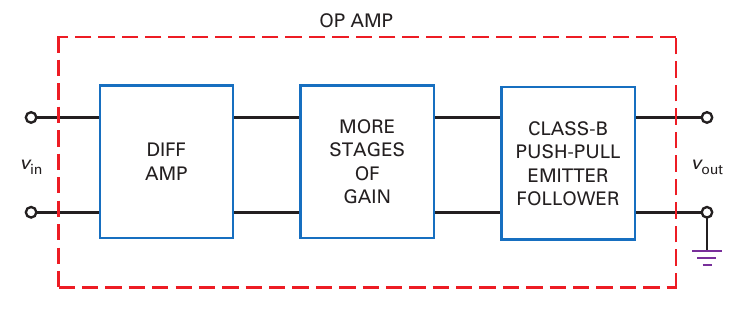
\includegraphics[width=0.7\linewidth]{pic/fig:16.01}
	\caption{Diagram blok dari op amp}
	\label{fig:16.01}
\end{figure}

Tidak semua op amp didesain seperti pada Gambar \ref{fig:16.01}. Misalkan, beberapa op amp tidak memiliki\textit{ Class-B push-pull output}, dan ada juga yang memiliki \textit{double-ended output}. Selain itu, op amp tidak sesederhana seperti yang ditunjukkan oleh Gambar \ref{fig:16.01}. Disain internal dari monolithic op amp sangatlah rumit, menggunakan ribuan transistor sebagai \textit{current mirror}, \textit{active load}, dan inovasi lainnya yang tidak mungkin ada di disain diskrit. Namun kita cukupkan sesuai dengan kebutuhan kita bahwa Gambar \ref{fig:16.01} menekankan pada dua fitur yang penting yaitu \textit{differential input} dan \textit{single-ended output}.

\begin{figure}
	\centering
	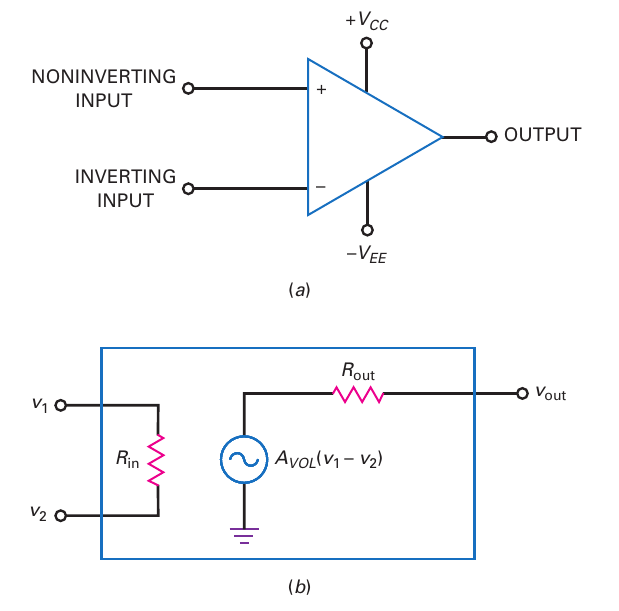
\includegraphics[width=0.7\linewidth]{pic/fig:16.02}
	\caption{(a) Simbol skematik dari op amp; (b) rangkaian ekivalen dari op amp}
	\label{fig:16.02}
\end{figure}

Gambar \ref{fig:16.02} adalah simbol skematik dari op amp. Pada gambar tersebut terdapat \textit{noninverting input}, \textit{inverting input} dan \textit{single-ended output}. Idealnya, simbol ini menjelaskan bahwa \textit{amplifier} memiliki \textit{voltage gain} yang tak berhingga, impedansi \textit{input} tak berhingga, dan impedansi \textit{output} nol. Op amp ideal merepresentasikan \textit{voltage amplifier} / penguat tegangan yang ideal dan ini sering disebut sebagai \textbf{voltage-controlled voltage source (VCVS)}. Kita dapat menggambarkan sebuah VCVS seperti pada Gambar \ref{fig:16.02}b, yang mana $ R_{in} $ adalah tak berhingga dan $ R_{out} $ adalah nol.

\begin{figure}
	\centering
	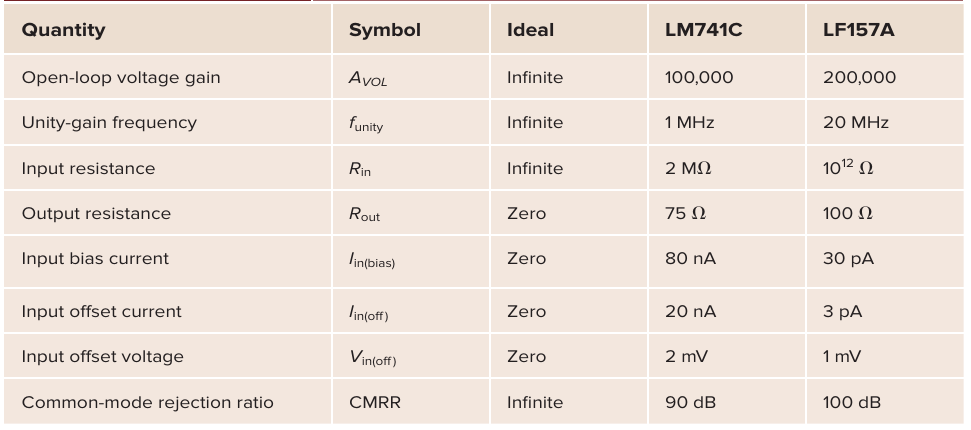
\includegraphics[width=\linewidth]{pic/tab:16.01}
	\caption{Ciri khas op amp}
	\label{tab:16.01}
\end{figure}

Gambar \ref{tab:16.01} menunjukkan ringkasan dari ciri khas atau karakteristik op amp. Op amp ideal memiliki \textit{voltage gain} yang tak berhingga, \textit{unity-gain frequency} yang tak berhingga, impedansi \textit{input} yang tak berhingga, dan CMRR yang tak berhingga. Op amp ideal juga memiliki resistansi \textit{output} yang nol, arus bias yang nol, dan arus offset yang nol. Seperti ini seharusnya op amp itu dibuat, jika mereka bisa. Namun apa yang mampu mereka buat hanyalah mendekati nilai ideal tersebut.

Sebagai contoh, LM741C dari Gambar \ref{tab:16.01} adalah op amp standar yang telah tersedia sejak 1960-an. Karaktistiknya adalah minimum dari dari apa yang kita harapkan dari monolithic ap amp. LM741C memiliki \textit{voltage gain} sebesar 100.000, \textit{unity-gain frequency} sebesar 1 MHz, impedansi \textit{input} sebesar 2 M$\Omega$, dan seterusnya. Karena \textit{voltage gain} sangat besar, offset input dapat dengan mudah membuat op amp bersaturasi. Hal ini lah mengapa kita membutuhkan komponen eksternal antara \textit{input} dan \textit{output} op amp untuk menstabilkan \textit{voltage gain}. Contohnya, di banyak aplikasi, \textit{negative feedback} digunakan untuk menyesuaikan \textit{overall voltage gain} ke nilai yang jauh lebih rendah sebagai ganti dari \textit{stable linear operation}.

Ketika tidak ada \textit{feedback} (atau \textit{loop}) yang digunakan, \textit{voltage gain} bernilai maksimum dan disebut dengan \textit{open-loop voltage gain}, yang dinotasikan dengan $ A_{VOL} $. Pada Gambar \ref{tab:16.01}, terlihat bahwa $ A_{VOL} $ dari LM741C adalah 100.000. Meskipun bukan tak berhingga, \textit{open-loop voltage gain} ini sangat besar. Contohnya, sebuah \textit{input} sebesar 10 $\mu$V menghasilkan \textit{output} 1 V. Karena \textit{open-loop voltage gain} sangat besar, kita dapat menggunakan \textit{heavy negative feedback} untuk meningkatkan performa keseluruhan dari rangkaian.

741C memiliki \textit{unity-gain frequency} sebesar 1 MHz. Artinya kita bisa menggunakan \textit{voltage gain} hingga 1 MHz. 741C memiliki resistansi \textit{input} sebesar 2 M$\Omega$, resistansi \textit{output} sebesar 75 $\Omega$, arus \textit{bias} \textit{input} sebesar 80 nA, arus \textit{offset} \textit{input} sebesar 20 nA, teganan \textit{offset output} sebesar 2 mV, dan CMRR sebesar 90 dB.

Ketika dibutuhkan resistansi input yang lebih besar, seorang \textit{engineer} dapat menggunakan \textbf{BIFET op amp}. Op amp jenis ini menggabungkan JFET dan transistor bipolar pada \textit{chip} yang sama. JFET digunakan di \textit{input stage} untuk mendapatkan arus \textit{bias input} dan arus \textit{offset input} yang lebih kecil. Transistor bipolar digunakan di \textit{stage} setelahnya untuk mendapatkan lebih banyak \textit{voltage gain}.

LF157A adalah salah satu contoh dari BIFET op amp. Seperti yang ditunjukkan oleh Gambar \ref{tab:16.01}, arus \textit{bias input} hanya sebesar 30 pA, dan resistansi \textit{input} sebesar $ 10^{12} $ $\Omega$. LF157A memiliki \textit{voltage gain} sebesar 200.000 dan \textit{unity-gain frequency} sebesar 20 MHz. Dengan menggunakan op amp ini, kita bisa mendapatkan \textit{voltage gain} hingga 20 MHz.


\section{Op Amp 741}

Pada tahun 1965, Fairchild Semiconductor memperkenalkan $\mu$A709, monolithic ap amp pertama yang banyak digunakan. Meskipun sukses, op amp generasi pertama memiliki banyak kekurangan. Hal ini yang melatarbelakangi terciptanya op amp $\mu$A741. Karena tidak mahal dan mudah digunakan, op amp $\mu$741 telah sukses besar. Desain 741 yang lain telah muncul dari berbagai manufaktur. Sebagai contoh, ON Semiconductor menghasilkan MC1741, Texas Instruments menghasilkan LM741, dan Analog Devices menghasilkan AD741. Semua monolithic op amp ini ekivalen dengan $\mu$A741 karena mereka memiliki spesifikasi yang sama di \textit{datasheet} mereka. Agar lebih mudah, kebanyak orang menghilangkan awalan dan lebih suka dengan istilah 741 saja.


\subsection{Standar Industri}

741 telah menjadi standar industri. Sebagai aturan, pertama kali kalian harus mencobanya di desain kalian. Jika kalian tidak dapat memenuhi spesifikasi desain dengan menggunakan 741, maka kalian gunakan op amp yang lebih baik. Karena ini standar, kita akan menggunakan 741 sebagai \textit{basic device} dalam diskusi kita ini. Ketika kalian telah paham dengan 741, kalian bisa mempelajari op amp lainnya.

741 memiliki berbagai nomor versi yang berbeda, 741, 741A, 741C, 741E, dan 741N. Perbedaannya adalah di bagian \textit{voltage gain}, \textit{temperature range}, \textit{noise level}, dan karakteristik-karakteristik lainnya. 741C (C artinya \textit{commercial grade}) adalah yang lebih murah dan paling banyak digunakan. 741C memiliki \textit{open-loop voltage gain} sebesar 100.000, impedansi \textit{input} sebesar 20 M$\Omega$, dan impedansi \textit{output} sebesar 75 $\Omega$. Gambar \ref{fig:16.03} menunjukkan 3 \textit{package style} yang populer dan \textit{pinout}-nya.

\begin{figure}
	\centering
	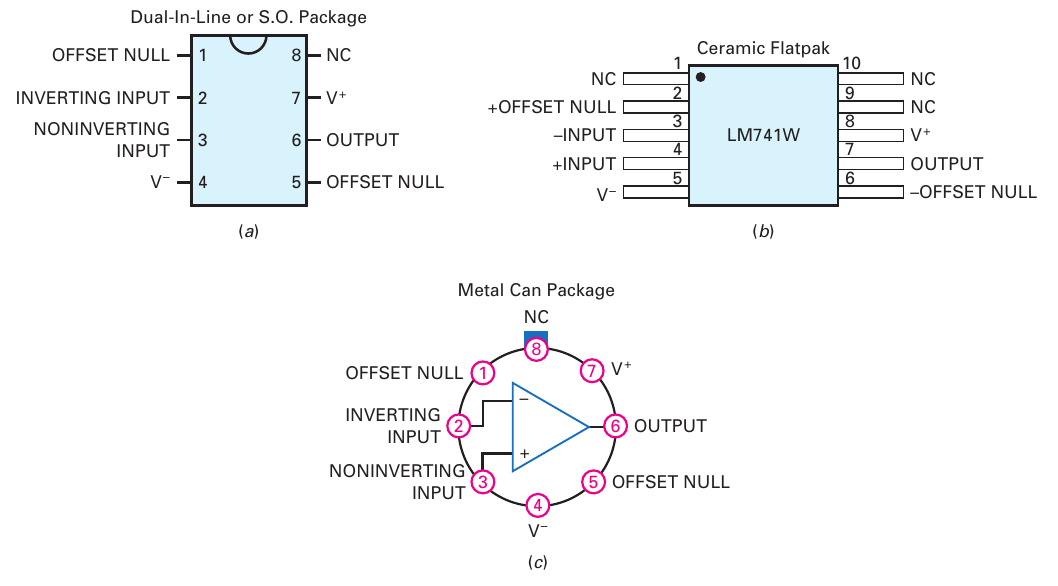
\includegraphics[width=\linewidth]{pic/fig:16.03}
	\caption{741 package stylke}
	\label{fig:16.03}
\end{figure}


\subsection{Input Diff Amp}

Gambar \ref{fig:16.04} adalah skematik diagram dari 741 yang disederhanakan. Rangkaian ini ekivalen dengan 741 dan banyak op amp generasi selanjutnya. Kalian tidak perlu memahami setiap detilnya tentang desain rangkaian ini, tapi kalian harus memiliki ide dasar dari bagaimana rangkaian ini bekerja.

\textit{Input stage} yang digunakan adalah diff amp ($ Q_1 $ dan $ Q_2 $). Pada 741, $ Q_{14} $ adalah sumber arus yang menggantikan \textit{tail resistor}. $ R_2 $, $ Q_{13} $, dan $ Q_{14} $ adalah arus mirror (\textit{current mirror}) yang menghasilkan arus \textit{tail} untuk $ Q_1 $ dan $ Q_2 $. Alih-alih menggunakan resistor biasa sebagai resistor \textit{collector} diff amp, 741 menggunakan \textit{active-load} resistor. \textit{Active-load} $ Q_4 $ ini bertindak seperti sumber arus dengan impedansi yang sangat tinggi. Karenanya, \textit{voltage gain} dari diff amp jauh lebih besar daripada dengan menggunakan \textit{passive-load} resistor.

\begin{figure}
	\centering
	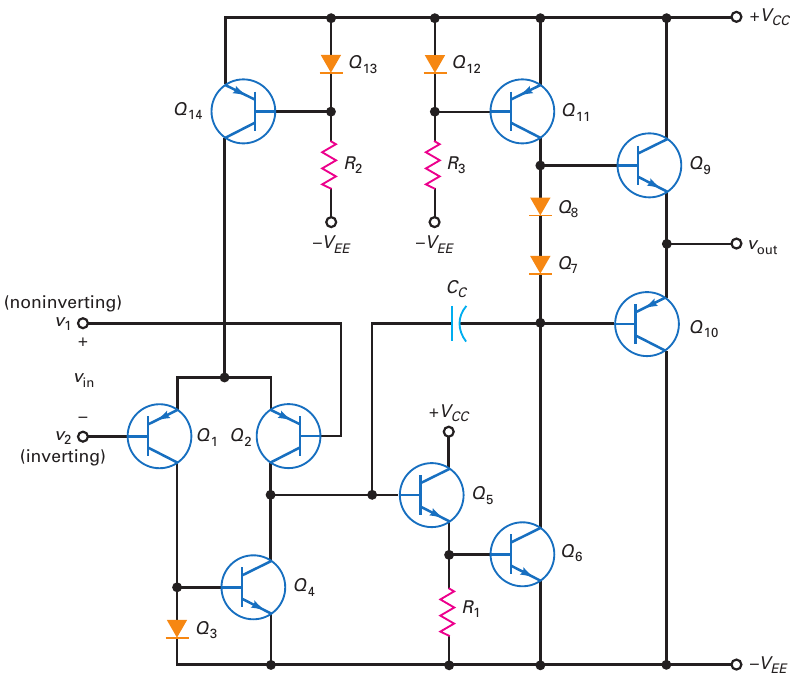
\includegraphics[width=\linewidth]{pic/fig:16.04}
	\caption{Skematik diagram 741 yang disederhanakan}
	\label{fig:16.04}
\end{figure}

Sinyal yang dikuatkan dari diff amp akan men-\textit{drive} \textit{base} $ Q_5 $, sebuah \textit{emitter follower}. Pada \textit{stage} ini, level impedansi dinaikkan untuk menghindari pembebanan diff amp. Sinyal yang keluar dari $ Q_5 $ menuju $ Q_6 $. Dioda $ Q_7 $ dan $ Q_8 $ adalah bagian dari bias untuk \textit{final stage}. $ Q_{11} $ adalah \textit{active-load} resistor untuk $ Q_6 $. Sehingga, $ Q_6 $ dan $ Q_{11} $ seperti \textit{CE driver stage} dengan \textit{voltage gain} yang sangat besar. Seperti yang telah dijelaskan pada bab sebelumnya, simbol dioda terkadang digunakan ketika \textit{base} transistor adalah dihubung-singkat ke \textit{collector}. Contohnya, $ Q_3 $ sebenarnya adalah transistor dengan base-collectornya terhubung singkat dan bekerja seperti dioda.


\subsection{Final Stage}

Sinyal yang dikuatkan keluar dari \textit{CE drive stage} ($ Q_6 $) menuju ke \textit{final stage}, yang berupa \textit{Class-B push-pull emitter follower} ($ Q_9 $ dan $ Q_{10} $). Karena \textit{split supply} (tegangan +$ V_{CC} $ dan -$ V_{EE} $), \textit{quiescent output} idealnya bernilai 0 V saat tegangan \textit{input} bernilai nol.

Ketika $ v_1 $ lebih besar daripada $ v_2 $, tegangan \textit{input} $ v_{in} $ menghasilkan tegangan \textit{output} positif. Ketika $ v_2 $ lebih besar daripada $ v_1 $, tegangan input $ v_{in} $ menghasilkan tegangan \textit{output} negatif $ v_{out} $. Idealnya, $ v_{out} $ bisa positif seperti +$ V_{CC} $ dan negatif seperti -$ V_{EE} $ sebelum \textit{clipping} terjadi. \textit{Output swing} normalnya antara 1 hingga 2 V dari masing-masing tegangan \textit{supply} karena teganan drop di dalam 741.


\subsection{Active Loading}
	
	\backmatter
	% bibliography, glossary and index would go here.
	
\end{document}